\documentclass[tikz,border=3pt]{standalone}
\usepackage{newtxtext,newtxmath}
\usetikzlibrary{arrows.meta}
\definecolor{paperink}{HTML}{3F4852}
\definecolor{paperblue}{HTML}{2F6DB0}
\definecolor{paperred}{HTML}{C83E4D}
\definecolor{papergreen}{HTML}{2E8B57}
\definecolor{papergray}{HTML}{F1F3F5}
\begin{document}
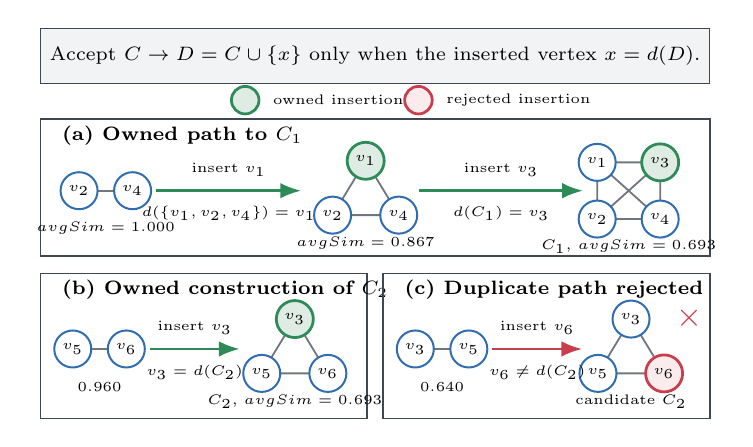
\begin{tikzpicture}[
  font=\scriptsize,
  >=Latex,
  vertex/.style={circle, draw=paperblue, fill=white, line width=0.72pt,
    minimum size=4.7mm, inner sep=0pt, font=\tiny},
  inserted/.style={vertex, draw=papergreen, fill=papergreen!16, line width=1.0pt},
  rejected/.style={vertex, draw=paperred, fill=paperred!10, line width=1.0pt},
  edge/.style={draw=paperink!75, line width=0.65pt},
  owned/.style={->, draw=papergreen, line width=1.0pt},
  duplicate/.style={->, draw=paperred, line width=1.0pt},
  paneltitle/.style={font=\scriptsize\bfseries, anchor=west},
  note/.style={font=\tiny, align=center},
  rule/.style={draw=paperink, fill=papergray, line width=0.6pt,
    minimum width=84mm, minimum height=7mm, align=center}
]

% Canonical rule shared by all panels.
\node[rule] at (4.20,1.18)
  {Accept $C\rightarrow D=C\cup\{x\}$ only when the inserted vertex $x=d(D)$.};
\node[inserted, minimum size=3.5mm] at (2.55,0.62) {};
\node[anchor=west, font=\tiny] at (2.78,0.62) {owned insertion};
\node[rejected, minimum size=3.5mm] at (4.75,0.62) {};
\node[anchor=west, font=\tiny] at (4.98,0.62) {rejected insertion};

% Panel (a): the owned path to C1.
\draw[paperink, line width=0.55pt] (-0.05,-1.36) rectangle (8.45,0.38);
\node[paneltitle] at (0.10,0.17) {(a) Owned path to $C_1$};

\begin{scope}[shift={(0.78,-0.53)}]
  \draw[edge] (-0.34,0)--(0.34,0);
  \node[vertex] at (-0.34,0) {$v_2$};
  \node[vertex] at ( 0.34,0) {$v_4$};
  \node[note] at (0,-0.48) {$\operatorname{avgSim}=1.000$};
\end{scope}

\begin{scope}[shift={(4.08,-0.53)}]
  \draw[edge] (0,0.38)--(-0.42,-0.31)--(0.42,-0.31)--cycle;
  \node[inserted] at (0,0.38) {$v_1$};
  \node[vertex] at (-0.42,-0.31) {$v_2$};
  \node[vertex] at ( 0.42,-0.31) {$v_4$};
  \node[note] at (0,-0.67) {$\operatorname{avgSim}=0.867$};
\end{scope}

\begin{scope}[shift={(7.42,-0.53)}]
  \coordinate (a) at (-0.40, 0.36);
  \coordinate (b) at (-0.40,-0.36);
  \coordinate (c) at ( 0.40, 0.36);
  \coordinate (d) at ( 0.40,-0.36);
  \draw[edge] (a)--(b)--(d)--(c)--cycle (a)--(d) (b)--(c);
  \node[vertex] at (a) {$v_1$};
  \node[vertex] at (b) {$v_2$};
  \node[inserted] at (c) {$v_3$};
  \node[vertex] at (d) {$v_4$};
  \node[note] at (0,-0.71) {$C_1$, $\operatorname{avgSim}=0.693$};
\end{scope}

\draw[owned] (1.42,-0.53)--(3.26,-0.53)
  node[midway,above=0.45mm,note] {insert $v_1$}
  node[midway,below=0.65mm,note] {$d(\{v_1,v_2,v_4\})=v_1$};
\draw[owned] (4.76,-0.53)--(6.84,-0.53)
  node[midway,above=0.45mm,note] {insert $v_3$}
  node[midway,below=0.65mm,note] {$d(C_1)=v_3$};

% Panel (b): accepted construction of C2.
\draw[paperink, line width=0.55pt] (-0.05,-3.42) rectangle (4.10,-1.58);
\node[paneltitle] at (0.10,-1.79) {(b) Owned construction of $C_2$};
\begin{scope}[shift={(0.70,-2.54)}]
  \draw[edge] (-0.34,0)--(0.34,0);
  \node[vertex] at (-0.34,0) {$v_5$};
  \node[vertex] at ( 0.34,0) {$v_6$};
  \node[note] at (0,-0.48) {$0.960$};
\end{scope}
\begin{scope}[shift={(3.18,-2.54)}]
  \draw[edge] (0,0.38)--(-0.42,-0.31)--(0.42,-0.31)--cycle;
  \node[inserted] at (0,0.38) {$v_3$};
  \node[vertex] at (-0.42,-0.31) {$v_5$};
  \node[vertex] at ( 0.42,-0.31) {$v_6$};
  \node[note] at (0,-0.67) {$C_2$, $\operatorname{avgSim}=0.693$};
\end{scope}
\draw[owned] (1.34,-2.54)--(2.48,-2.54)
  node[midway,above=0.45mm,note] {insert $v_3$}
  node[midway,below=0.65mm,note] {$v_3=d(C_2)$};

% Panel (c): alternative insertion creates C2 but is not owned.
\draw[paperink, line width=0.55pt] (4.30,-3.42) rectangle (8.45,-1.58);
\node[paneltitle] at (4.45,-1.79) {(c) Duplicate path rejected};
\begin{scope}[shift={(5.05,-2.54)}]
  \draw[edge] (-0.34,0)--(0.34,0);
  \node[vertex] at (-0.34,0) {$v_3$};
  \node[vertex] at ( 0.34,0) {$v_5$};
  \node[note] at (0,-0.48) {$0.640$};
\end{scope}
\begin{scope}[shift={(7.45,-2.54)}]
  \draw[edge] (0,0.38)--(-0.42,-0.31)--(0.42,-0.31)--cycle;
  \node[vertex] at (0,0.38) {$v_3$};
  \node[vertex] at (-0.42,-0.31) {$v_5$};
  \node[rejected] at ( 0.42,-0.31) {$v_6$};
  \node[font=\large, text=paperred] at (0.74,0.39) {$\times$};
  \node[note] at (0,-0.67) {candidate $C_2$};
\end{scope}
\draw[duplicate] (5.69,-2.54)--(6.83,-2.54)
  node[midway,above=0.45mm,note] {insert $v_6$}
  node[midway,below=0.65mm,note] {$v_6\neq d(C_2)$};

\end{tikzpicture}
\end{document}
